\pdfminorversion=4
\documentclass{beamer}
\usepackage[T1]{fontenc}
\usepackage[ngerman]{babel}
\usepackage[utf8]{inputenc}
\usepackage[babel,german=quotes]{csquotes}
\usepackage{amsmath,amsfonts,amssymb}
\usepackage{hyperref}
\usepackage{lmodern}

\usetheme{fau-4-3}

\usepackage[sort&compress,comma,super,square]{natbib}
%\bibliographystyle{apalike} % Or your specific bibliographystyle
\bibliographystyle{unsrtdin}
%\bibliographystyle{gerplain}


\title{cowbusconfig – Ansatz zur dezentralen Konfiguration von Gebäudeautomation}
\author[P. Kanzler, M. Zapf]{Patrick\,Kanzler \and Michael\,Zapf}
\date{23.09.2015}


\begin{document}
\frame{\titlepage}

%\section{cowbusconfig – Ansatz zur dezentralen Konfiguration von Gebaueudeautomation}
\begin{frame}
    \frametitle{Ziele und Ideen}

    \begin{itemize}
        \item dezentrale Organisation
        \item
        \item
        \item
        \item
    \end{itemize}
\end{frame}

\begin{frame}
    \frametitle{Regeln}

    \begin{itemize}
        \item 
        \item
        \item
        \item
        \item
        \item
    \end{itemize}
\end{frame}

\begin{frame}
    \frametitle{Konfigurationsnachrichten}

    \begin{itemize}
        \item
        \item
        \item
        \item
        \item
    \end{itemize}
\end{frame}

\begin{frame}
    \frametitle{Demo}
\end{frame}

\section{Q\&A}

\section{Vielen Dank für Ihre Aufmerksamkeit!}

%\begin{frame}[plain]
%    \center
%    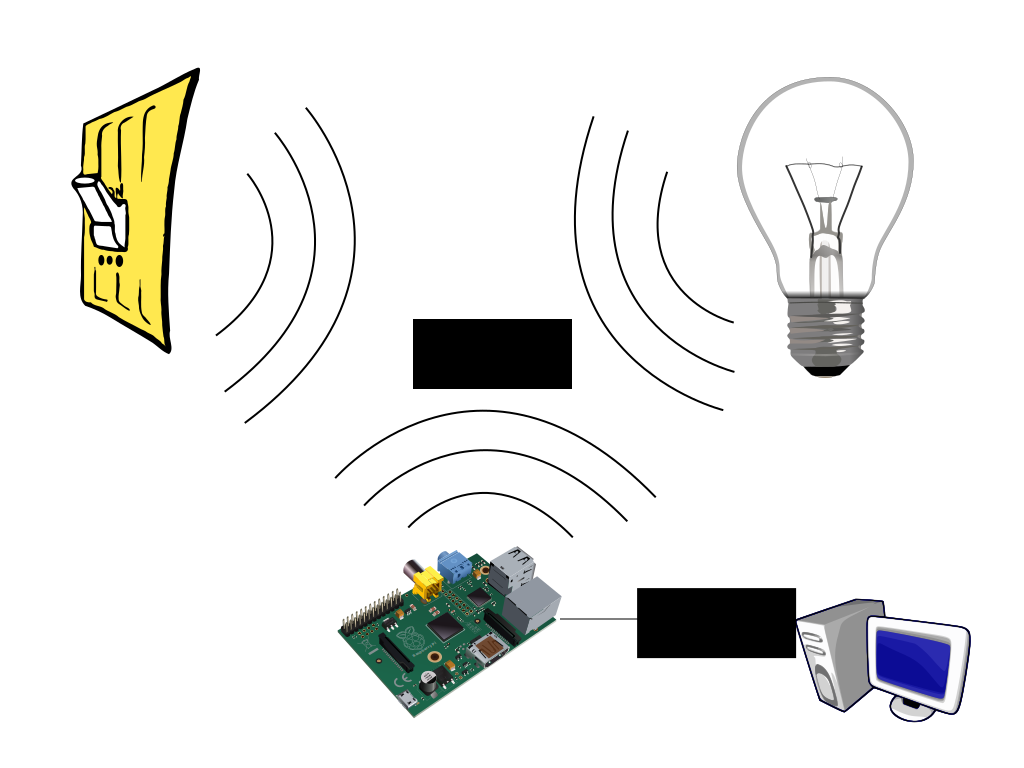
\includegraphics[scale=0.4]{img/system}
%\end{frame}


%\nocite*
%\bibliography{2015-09-cowconfig}{}

\end{document}

